\documentclass[11pt]{article}
\usepackage[T1]{fontenc}\usepackage{lmodern,amsmath,graphicx,geometry,microtype,caption}
\usepackage[hidelinks]{hyperref}\geometry{letterpaper,margin=1in}\pagestyle{empty}
\renewcommand{\thefigure}{S\arabic{figure}}\setcounter{figure}{8}
\begin{document}
\begin{figure}[!ht]\centering
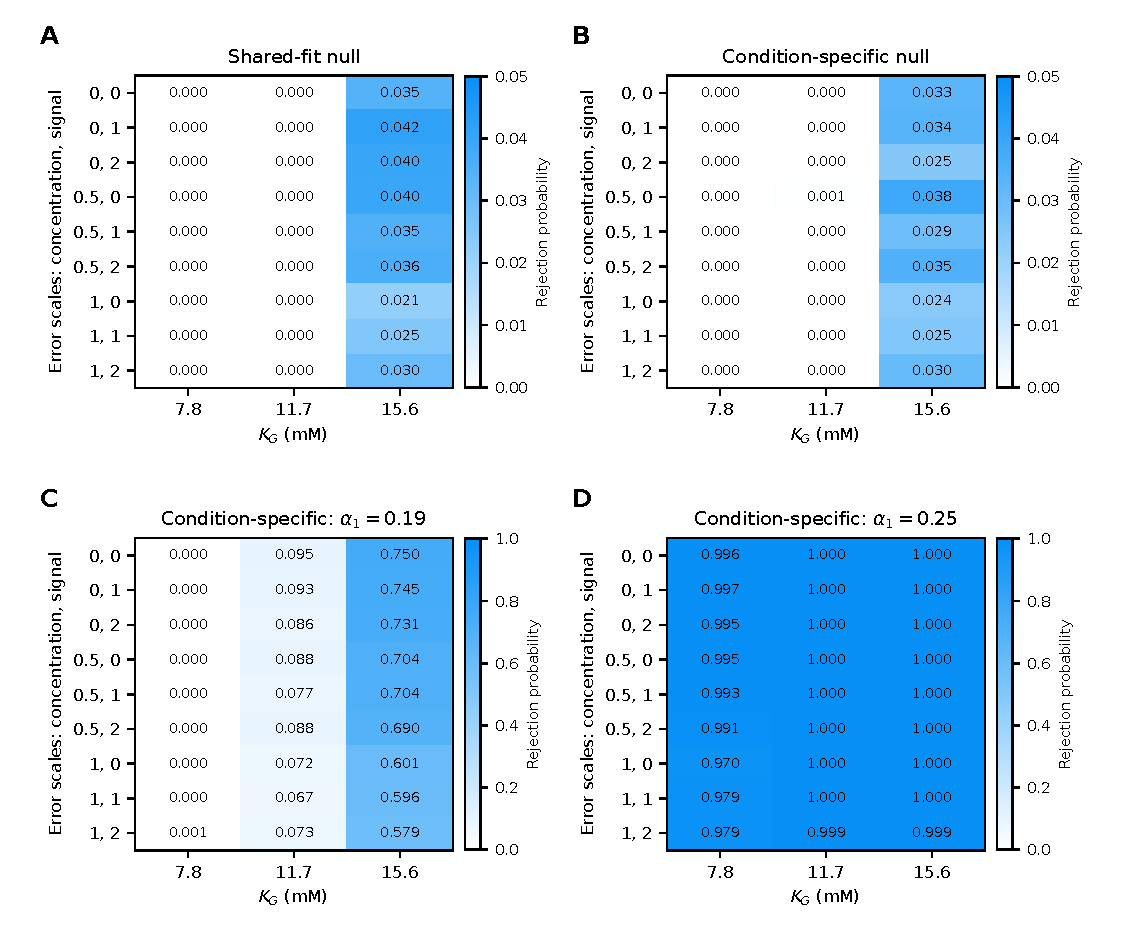
\includegraphics[width=\textwidth]{figure_inputs/nuisance_grid.pdf}
\caption{\textbf{All audited nuisance cells for the null and two alternative effects.} Each cell gives the rejection proportion from 2,000 independently evaluated trials after separate parametric calibration. Rows cross concentration-error scales $c=0,0.5,1$ with signal-error scales $s=0,1,2$; their physical error magnitudes are defined in S3 Appendix E5. (A--B) Shared and condition-specific fits under the $\alpha_1=0.17$ reference. (C--D) Condition-specific fits under $\alpha_1=0.19$ and 0.25. Null panels use a 0--0.05 color scale; alternative panels use 0--1. Printed values are rounded to three decimal places. These are a discrete sensitivity grid, not an interpolated continuous performance guarantee.}
\end{figure}
\end{document}
